%----------------------------------------------------------------------
% Problem 2

\begingroup
\allowdisplaybreaks

\newpage
\section{Problem 2}

\textbf{Exercise 4 in Section 3.6}

\subsection{Solution}

\textbf{NOTE: } \textit{I do not have any experience in seismology, please forgive any mistakes in technicalities when I try to explain this exercise in my own words. It helps me understand what is going on so I can set up the problem correctly.}
\newline

The forward problem in this exercise allows mechanical waves to propagate through a $16 \times 16$ meter grid where each square in the grid have some slowness value $s_{x,y}$ in units of \unit{\second\per\meter}. Stations around the grid record time of arrivals of the mechanical waves as they pass through one or multiple grid squares. The time it takes to pass through a path of squares is formulated below.

\begin{align*}
	t &= \int_l s\left(\bv{x}\right) dl \\
	\\
	&\approx \sum_{blocks} s_{block} \Delta l
\end{align*}


\subsubsection{Part A - Row and Column Scans Only}

$16$ row scans and $16$ column scans are utilized in this part in the exercise as shown in figure \ref{fig: prob2 part A row column scan viz}. 

\begin{figure}[h] 
	\centering
	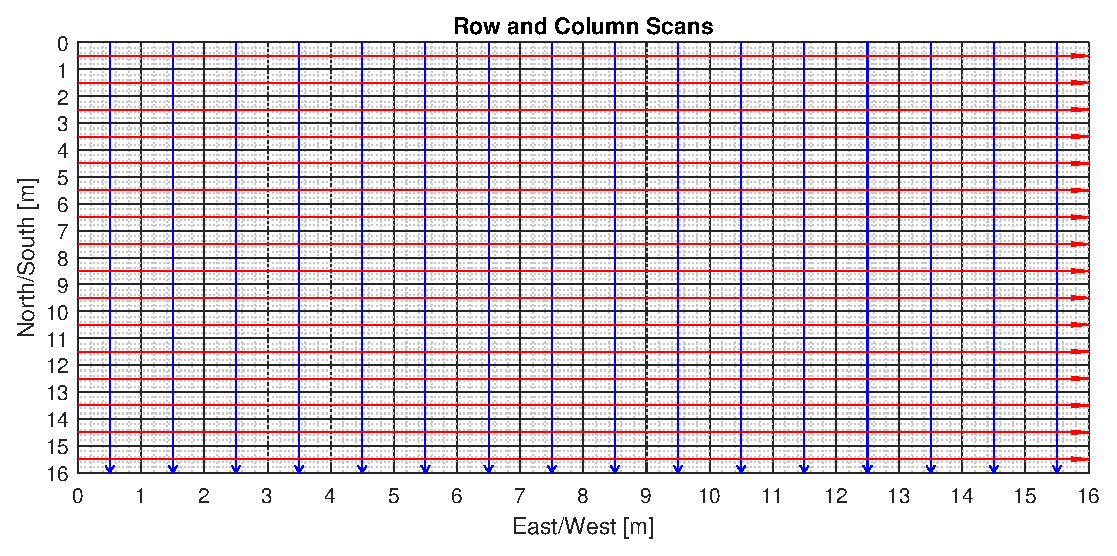
\includegraphics[width=0.65\textwidth]{./images/prob2_partA_scans_vizualization.eps}
	\caption{Row and Column Scan Visualization}
	\label{fig: prob2 part A row column scan viz}
\end{figure}
\FloatBarrier

This results in a total of $m = 32$ measurements. In an effort to estimate the slowness of each square in the grid, this results in a number of $n = 256$ model parameters. 

\begin{align*}
	\bv{d} \in \R^{32},\,\,\,\,\,\bv{m} \in \R^{256},\,\,\,\,\,G \in \R^{32 \times 256}
\end{align*}

The vector of measurement observations $\bv{d}$ is organized such that

\begin{align*}
	\bv{d} = \begin{bmatrix}
		t_{r,1} & t_{r,2} & \ldots & t_{r,16} & t_{c,1} & t_{c,2} & \ldots & t_{c,16}
	\end{bmatrix}^T
\end{align*}

where a $r$ subscript indicates a row can and a $c$ subscript indicates a column scan. The model parameters $\bv{m}$ are organized such that

\begin{align*}
	\bv{m} = \begin{bmatrix}
		s_{1,1} & s_{1,2} & \ldots & s_{1,16} & s_{2,1} & s_{2,2} & \ldots & s_{16,1} & \ldots & s_{16,16}
	\end{bmatrix}^T
\end{align*}

where the first subscript indicates the row, and the second subscript indicates the column. Each row of the model operator $G$ contain the distance traveled by the mechanical wave for each square in its path. Due to the large number of elements, a color map of the zeros and ones for this part of the problem as given instead in figure \ref{fig: prob2 part A model operator G}.

\begin{figure}[h] 
	\centering
	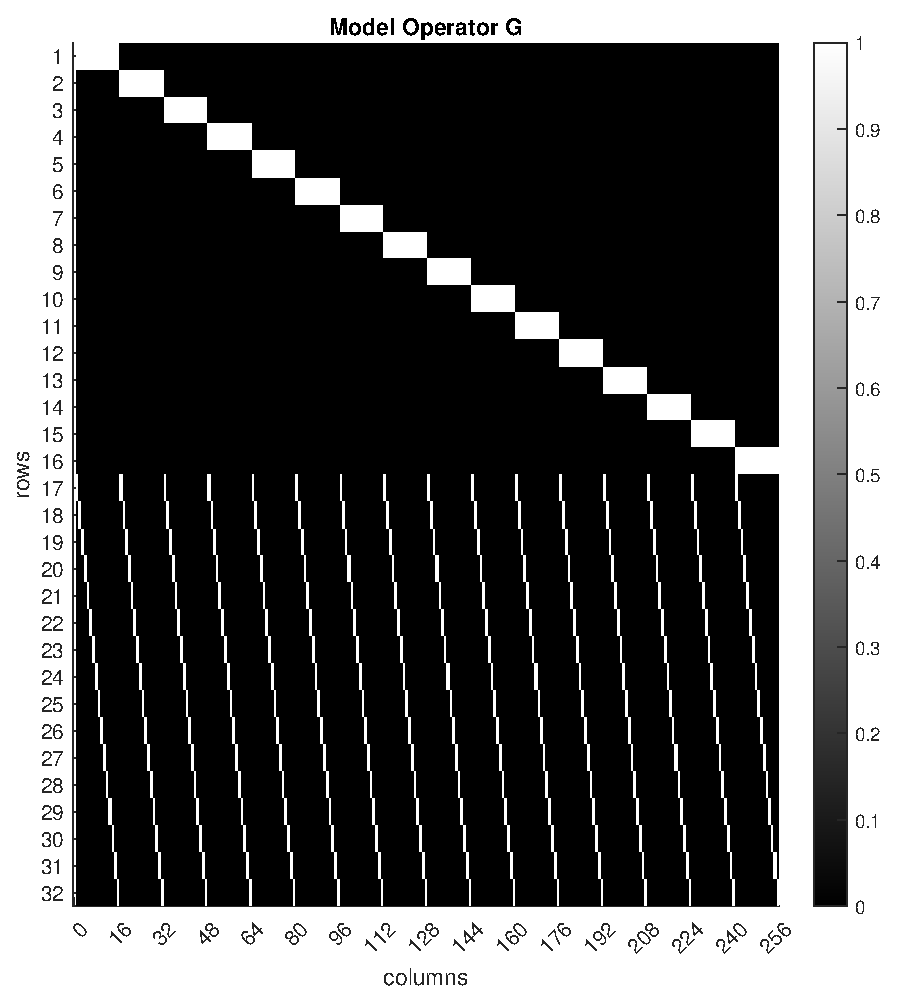
\includegraphics[width=0.65\textwidth]{./images/prob2_partA_model_operator_G.eps}
	\caption{Model Operator $G$}
	\label{fig: prob2 part A model operator G}
\end{figure}
\FloatBarrier

\textbf{Subpart A} \newline
Per \MATLAB, the rank of G is $31$. With $m = 32$ observations and $n = 256$ model parameters, the matrix of $G$ is not of full rank.
\newline

\textbf{Subpart B} \newline
This is the environment of "$p < m$ and $p < n$", in which both the data null space and model null space are nontrivial and the solution $\bv{m}^\dagger$ is the minimum length least squares solution. 

\begin{align*}
	m_{\dagger} = G^\dagger \bv{d} = V_p S_p^{-1} U_p^T \bv{d}
\end{align*}

Because $G$ is rank-deficient, there will be no exact solution. With $p = \textrm{rank}\left(G\right) = 31$ and $m = 32$, the dimensions of the data and model range and null spaces will are

\begin{align*}
	U_p \in \R^{32 \times 31},\, Vp \in \R^{256 \times 31}, \,\,\,\,\, U_0 \in \R^{32 \times 1}, \, V_0 \in R^{256 \times 225}
\end{align*}

such that it fits the form below.

\begin{align*}
	G = \begin{bmatrix} U_p & U_0 \end{bmatrix} \begin{bmatrix} S_p & 0 \\ 0 & 0 \end{bmatrix} \begin{bmatrix} V_p & V_0 \end{bmatrix}^T  
\end{align*}

Examples of vectors in each null space are provided in figure \ref{fig: prob2 part A null space examples}. Interpreting these patterns, the data null space vector appear to have small constant values for two groups of 16 elements. There isn't any useful data in this vector to assist in estimating the model parameters. Likewise, the example model null space vector contains mostly values close to zero which would not significantly alter a recovered if added.  

\begin{figure}[h] 
	\centering
	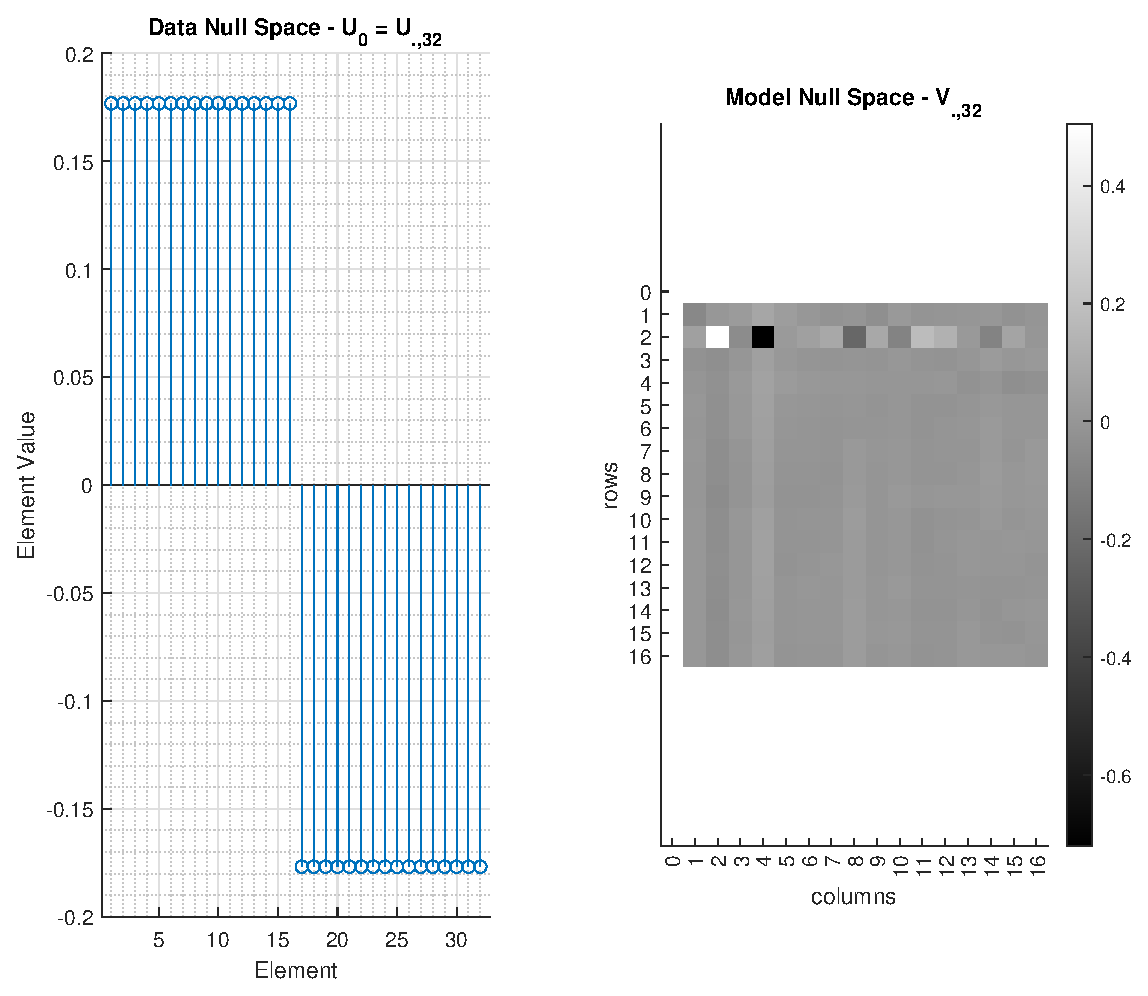
\includegraphics[width=0.85\textwidth]{./images/prob2_partA_null_space_examples.eps}
	\caption{Null Space Examples}
	\label{fig: prob2 part A null space examples}
\end{figure}
\FloatBarrier

The model resolution matrix is provided in figure \ref{fig: prob2 part A model resolution matrix}. 
 
\begin{figure}[h] 
	\centering
	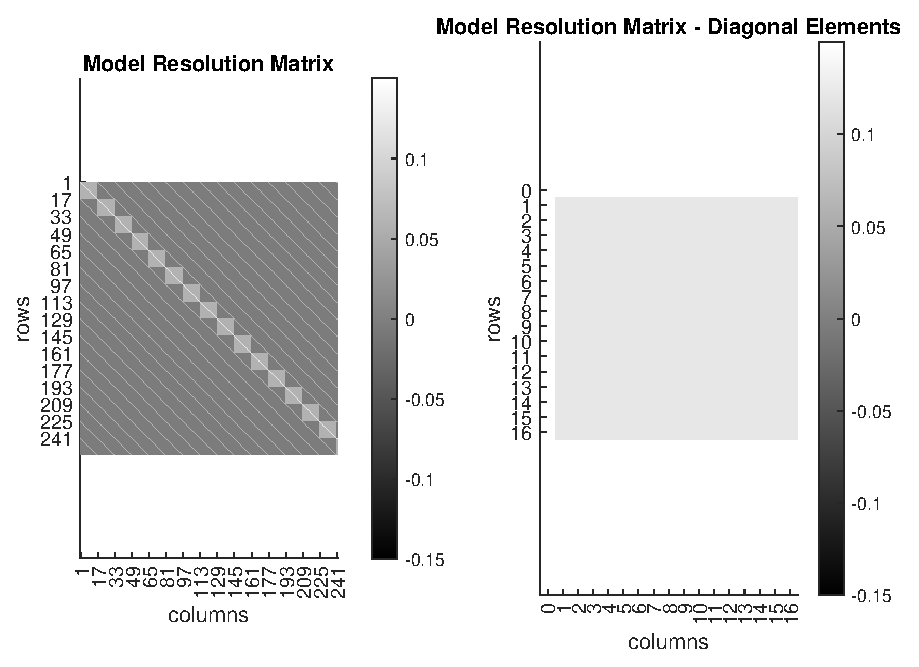
\includegraphics[width=0.85\textwidth]{./images/prob2_partA_model_resolution_matrix.eps}
	\caption{Model Resolution Matrix $R_m$}
	\label{fig: prob2 part A model resolution matrix}
\end{figure}
\FloatBarrier

Note that there are no diagonal elements which provide perfect model resolution. Each model parameter appears to be equally smeared. \newline

\textbf{Subpart C} \newline

Model parameters are computed using the \verb|pinv()| function in \MATLAB, and results are provided in figure \ref{fig: prob2 part A estimated model parameters}.

\begin{figure}[h] 
	\centering
	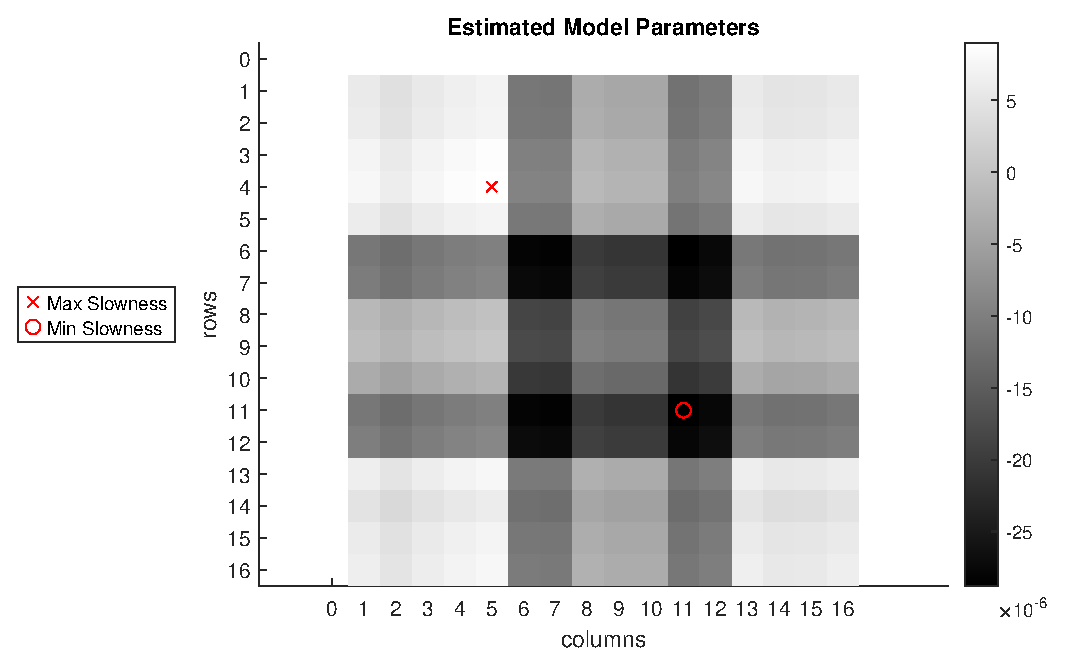
\includegraphics[width=0.85\textwidth]{./images/prob2_partA_estimated_model_parameters.eps}
	\caption{Estimated Model Parameters}
	\label{fig: prob2 part A estimated model parameters}
\end{figure}
\FloatBarrier

The maximum and minimum estimated slowness values are 

\begin{align*}
	s_{max} &= 8.971 \times 10^{-6} \, \unit{\second\per\meter} \\
	s_{min} &= -2.878 \times 10^{-5} \, \unit{\second\per\meter}
\end{align*}

which imply velocities of

\begin{align*}
	v_{max} &= 1878457.875 \, \unit{\meter\per\second} \\
	v_{min} &= -34130333.333 \, \unit{\meter\per\second}
\end{align*}

throughout the various square grids. 

\begin{figure}[h] 
	\centering
	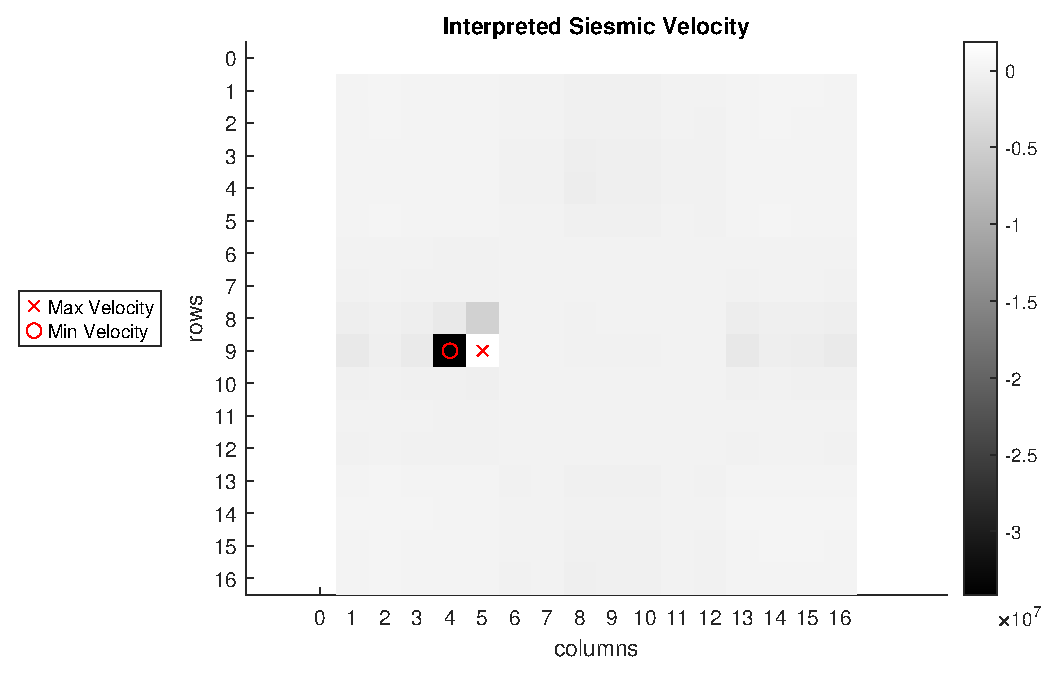
\includegraphics[width=0.85\textwidth]{./images/prob2_partA_seismic_velocity.eps}
	\caption{Interpreted Seismic Velocity}
	\label{fig: prob2 part A seismic velocity}
\end{figure}
\FloatBarrier

The maximum velocity square is in the $9^{th}$ row and $5^{th}$ column. \textit{Again, I do not study seismology}, but assuming that the dinosaur bones are related to the highest velocity we expect to find in our search space, then they must be located in the square with the highest velocity value.

Obviously, these velocities reported have no physical connection to reality. The estimated slowness parameters are incredibly small which results in huge velocities far beyond the expected $3000 \unit{\meter\per\second}$ velocity. This is perhaps a case when the minimum length model solution can be a hindrance to estimating meaningful parameters. \newline

\textbf{Subpart D} \newline

Given the dimensions of $V_0$, there are 225 example solutions that could fit the system of equations $G\bv{m} = \bv{d} = \bv{0}$. In fact, there are actually an infinite amount of example solutions which could comprise any linear combination of these 225 example model null space vectors. 

To demonstrate a "wild" model that can fit this solution, let's use a linear combination of three model null space vectors such that:

\begin{align*}
	\bv{m}_{wild} = 0.25 V_{.,32} + 0.50 V_{.,127} + 0.25 V_{.,183}
\end{align*}

Formulating this wild solution in \MATLAB to predict the resulting data produces the following results in figure \ref{fig: prob2 part A wild data and model}.

\begin{figure}[h] 
	\centering
	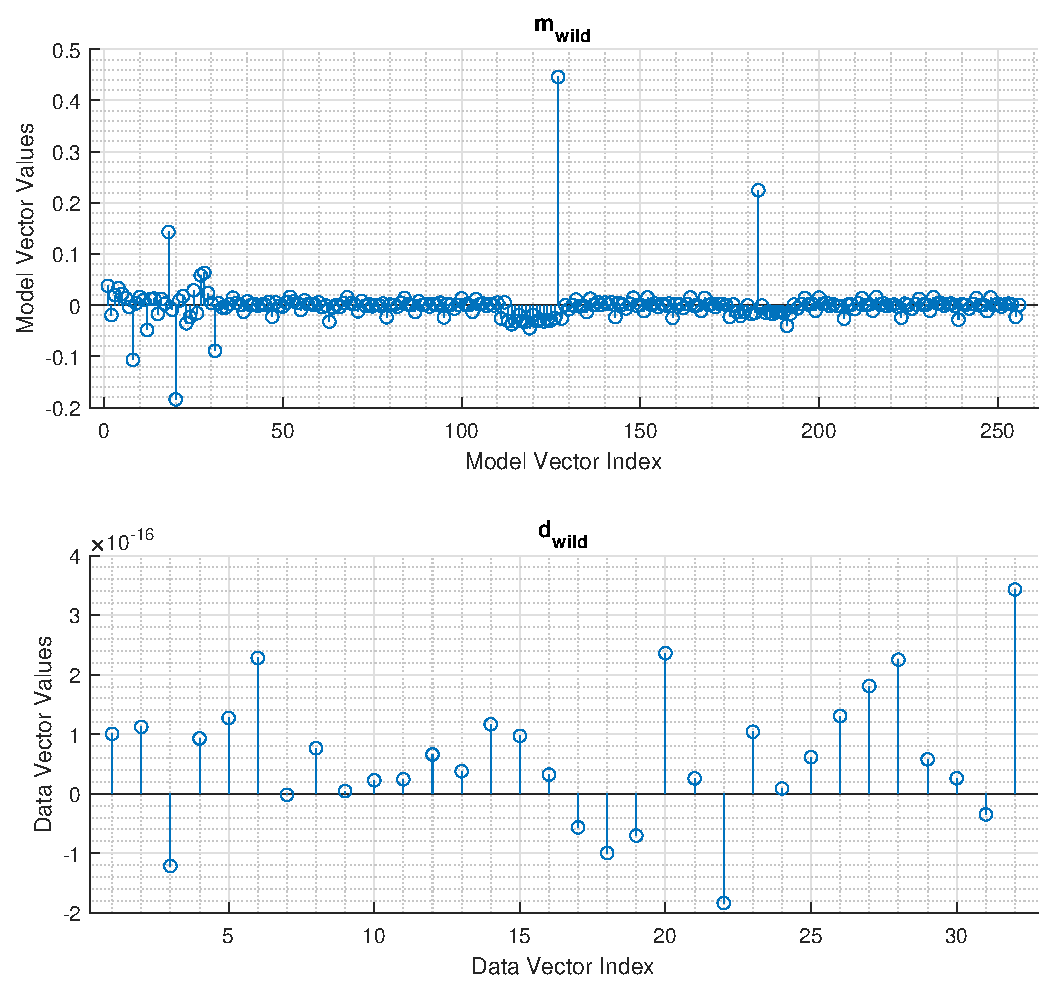
\includegraphics[width=0.85\textwidth]{./images/prob2_partA_wild_model_and_data.eps}
	\caption{Wild Model and Resulting Predicted Data}
	\label{fig: prob2 part A wild data and model}
\end{figure}
\FloatBarrier

Notice the scale of the values for the predicted data vector!


%--------------------------------------------------------------------
% Part B

\subsubsection{Part B - Adding in the Diagonal Scans}

$16$ row scans, $16$ column scans, and $62$ diagonal scans are utilized in this part in the exercise as shown in figure \ref{fig: prob2 part B row column scan viz}. 

\begin{figure}[h] 
	\centering
	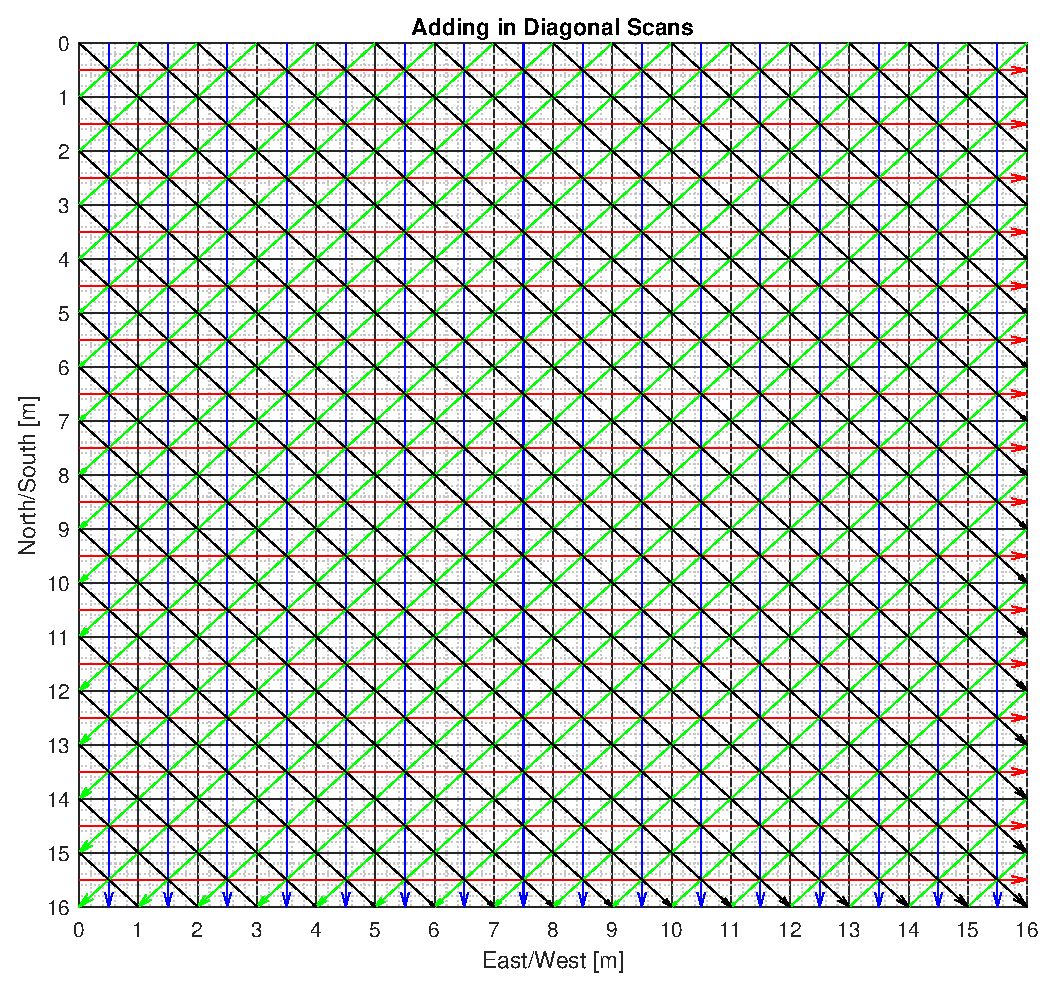
\includegraphics[width=0.65\textwidth]{./images/prob2_partB_scans_vizualization.eps}
	\caption{Adding the Diagonal Scans}
	\label{fig: prob2 part B row column scan viz}
\end{figure}
\FloatBarrier

This results in a total of $m = 94$ measurements. In an effort to estimate the slowness of each square in the grid, this results in a number of $n = 256$ model parameters. 

\begin{align*}
	\bv{d} \in \R^{94},\,\,\,\,\,\bv{m} \in \R^{256},\,\,\,\,\,G \in \R^{94 \times 256}
\end{align*}

Due to the large number of elements, a color map of the zeros and ones for this part of the problem as given instead in figure \ref{fig: prob2 part B model operator G}.

\begin{figure}[h] 
	\centering
	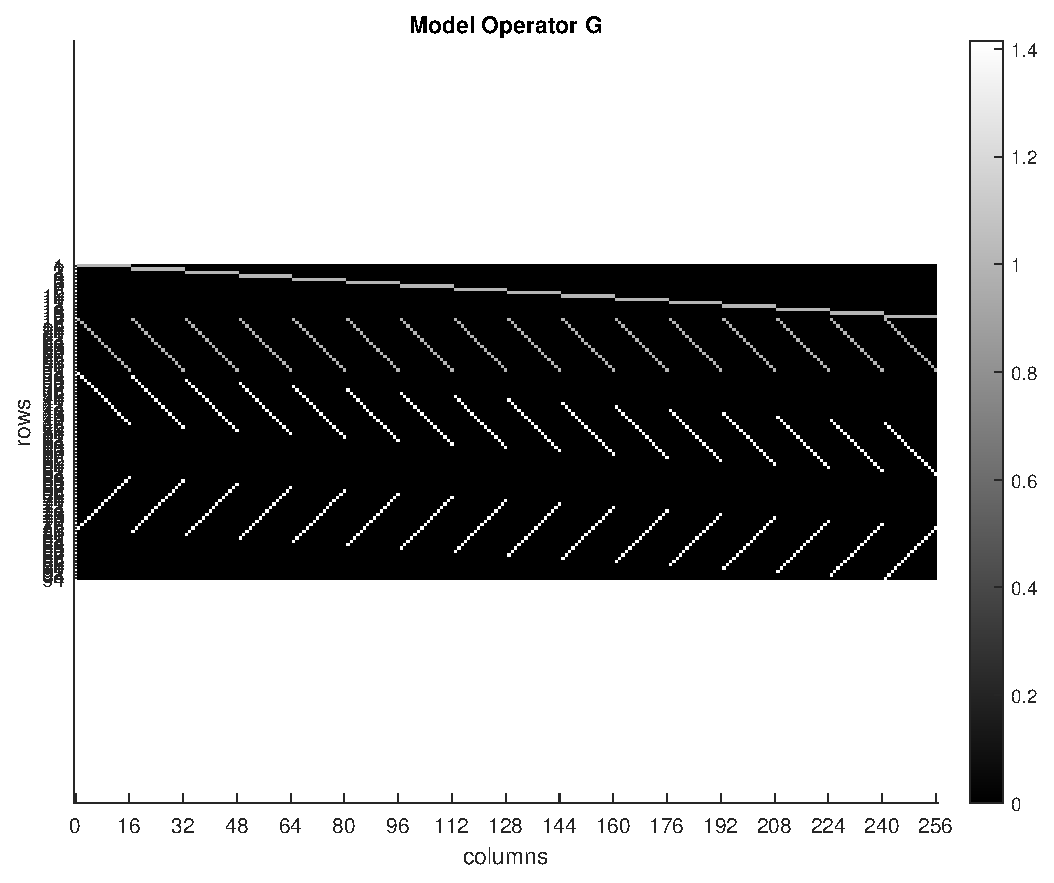
\includegraphics[width=0.65\textwidth]{./images/prob2_partB_model_operator_G.eps}
	\caption{Model Operator $G$}
	\label{fig: prob2 part B model operator G}
\end{figure}
\FloatBarrier

\textbf{Subpart A} \newline
Per \MATLAB, the rank of G is $87$. With $m = 94$ observations and $n = 256$ model parameters, the matrix of $G$ is not of full rank.
\newline

\textbf{Subpart B} \newline
This is the environment of "$p < m$ and $p < n$", in which both the data null space and model null space are nontrivial and the solution $\bv{m}^\dagger$ is the minimum length least squares solution. 

\begin{align*}
	m_{\dagger} = G^\dagger \bv{d} = V_p S_p^{-1} U_p^T \bv{d}
\end{align*}

Because $G$ is rank-deficient, there will be no exact solution. With $p = \textrm{rank}\left(G\right) = 97$ and $m = 94$, the dimensions of the data and model range and null spaces will are

\begin{align*}
	U_p \in \R^{94 \times 87},\, Vp \in \R^{256 \times 87}, \,\,\,\,\, U_0 \in \R^{94 \times 7}, \, V_0 \in R^{256 \times 169}
\end{align*}

such that it fits the form below.

\begin{align*}
	G = \begin{bmatrix} U_p & U_0 \end{bmatrix} \begin{bmatrix} S_p & 0 \\ 0 & 0 \end{bmatrix} \begin{bmatrix} V_p & V_0 \end{bmatrix}^T  
\end{align*}

Examples of vectors in each null space are provided in figure \ref{fig: prob2 part B null space examples}. Interpreting these patterns, the data null space vector appears to have some sort of sinusoidal wave with a small amplitude which could perhaps be interpreted as noise filtered out of the solution. I suspect that there isn't any useful data in this vector to assist in estimating the model parameters as there is nothing about the arrival of mechanical waves that be sinusoidal. Likewise, the example model null space vector contains mostly values close to zero which would not significantly alter a recovered if added.  

\begin{figure}[h] 
	\centering
	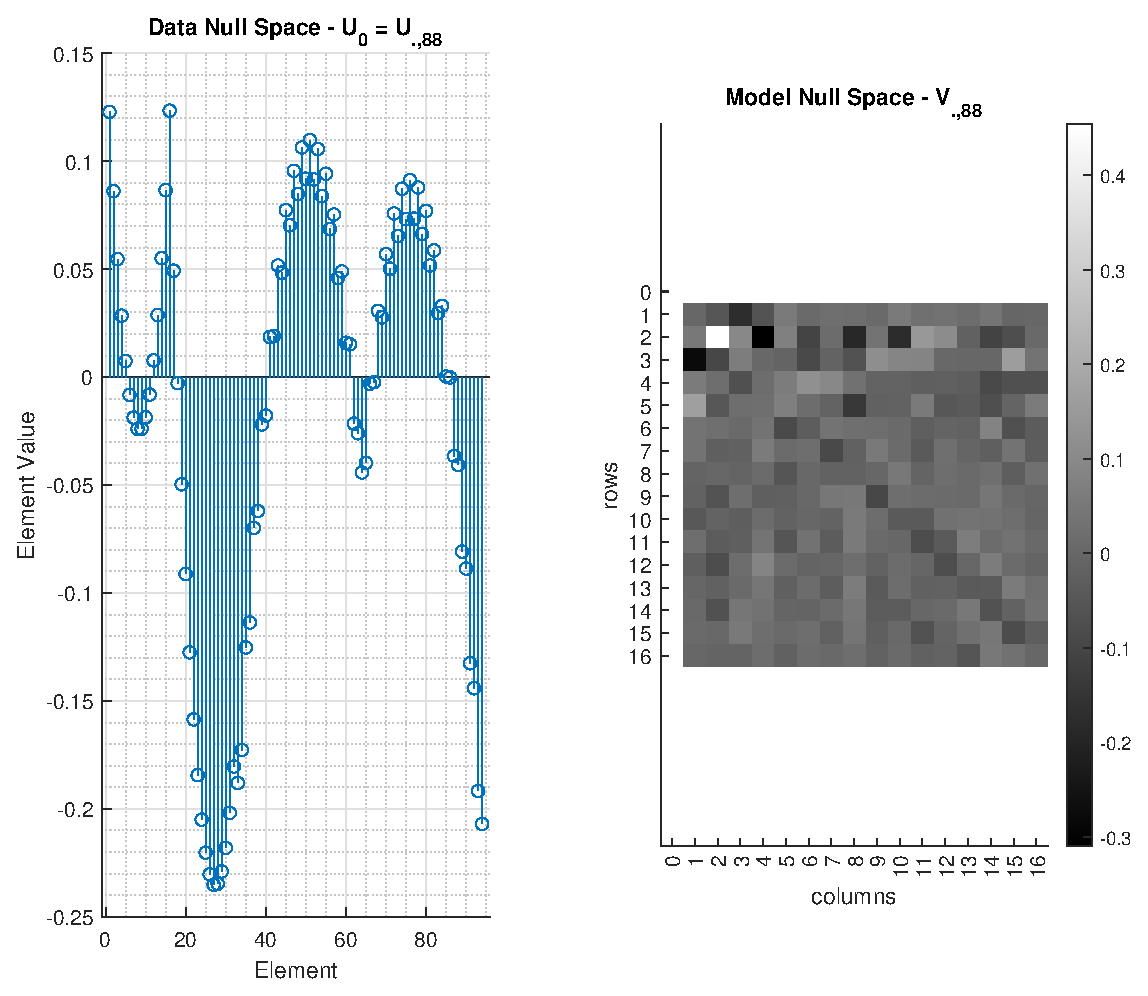
\includegraphics[width=0.85\textwidth]{./images/prob2_partB_null_space_examples.eps}
	\caption{Null Space Examples}
	\label{fig: prob2 part B null space examples}
\end{figure}
\FloatBarrier

The model resolution matrix is provided in figure \ref{fig: prob2 part B model resolution matrix}. 

\begin{figure}[h] 
	\centering
	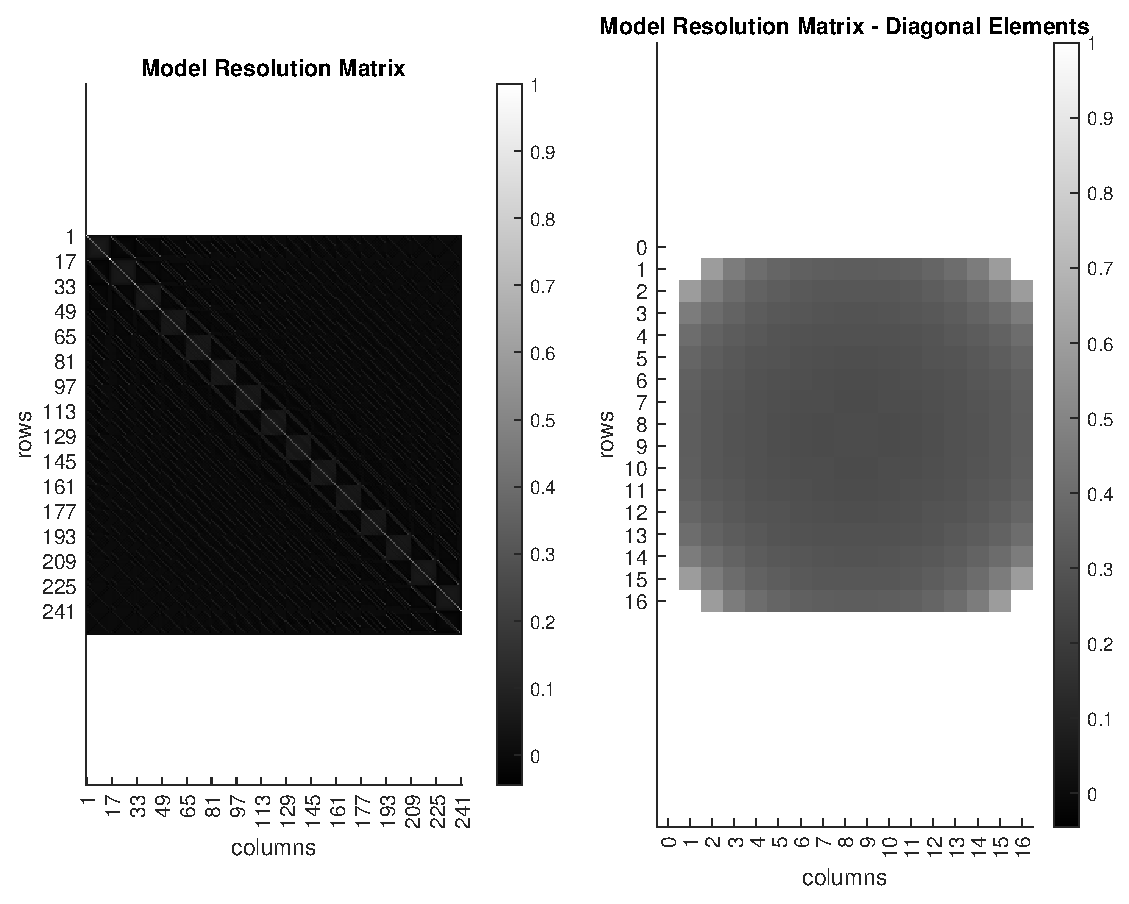
\includegraphics[width=0.85\textwidth]{./images/prob2_partB_model_resolution_matrix.eps}
	\caption{Model Resolution Matrix $R_m$}
	\label{fig: prob2 part B model resolution matrix}
\end{figure}
\FloatBarrier

Each "corner" parameter in the $16 \times 16$ grid has perfect resolution. I suspect this is because in the diagonal scans, there are some measurements which the corner square is the only activated square for that measurement. All other parameters are subject to some amount of smearing. \newline

\textbf{Subpart C} \newline

Model parameters are computed using the \verb|pinv()| function in \MATLAB, and results are provided in figure \ref{fig: prob2 part B estimated model parameters}.

\begin{figure}[h] 
	\centering
	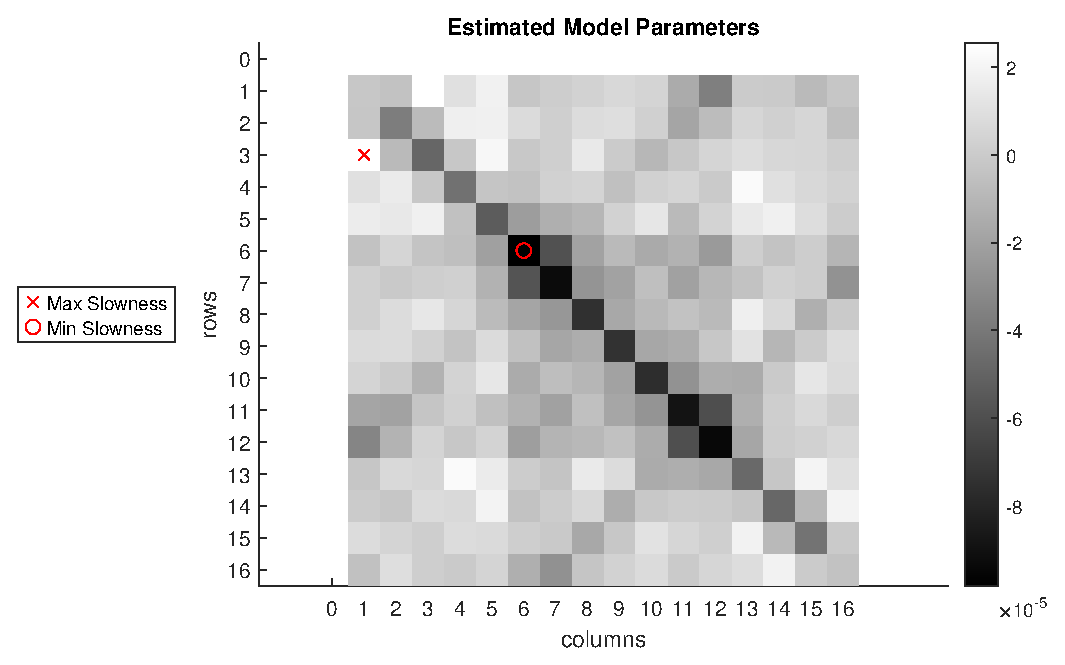
\includegraphics[width=0.85\textwidth]{./images/prob2_partB_estimated_model_parameters.eps}
	\caption{Estimated Model Parameters}
	\label{fig: prob2 part B estimated model parameters}
\end{figure}
\FloatBarrier

The maximum and minimum estimated slowness values are 

\begin{align*}
	s_{max} &= 2.548 \times 10^{-5} \, \unit{\second\per\meter} \\
	s_{min} &= -9.823 \times 10^{-5} \, \unit{\second\per\meter}
\end{align*}

which imply velocities of

\begin{align*}
	v_{max} &= 90870796.137 \, \unit{\meter\per\second} \\
	v_{min} &= -7250593.614 \, \unit{\meter\per\second}
\end{align*}

throughout the various square grids. 

\begin{figure}[h] 
	\centering
	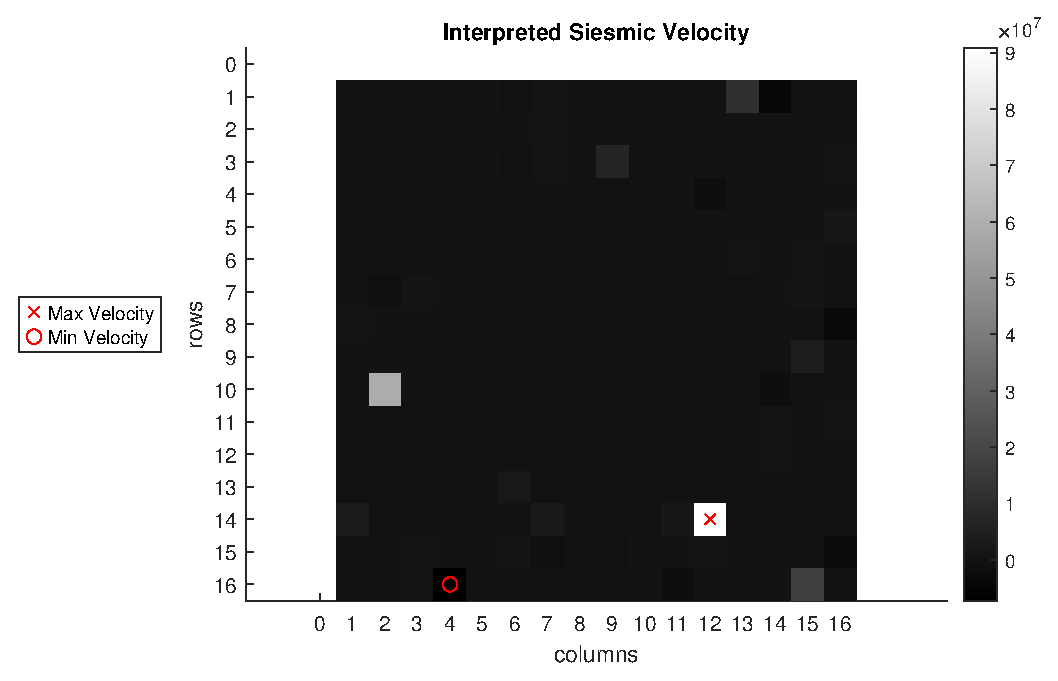
\includegraphics[width=0.85\textwidth]{./images/prob2_partB_seismic_velocity.eps}
	\caption{Interpreted Seismic Velocity}
	\label{fig: prob2 part B seismic velocity}
\end{figure}
\FloatBarrier

The maximum velocity square is in the $14^{th}$ row and $12^{th}$ column. \textit{Again, I do not study seismology}, but assuming that the dinosaur bones are related to the highest velocity we expect to find in our search space, then they must be located in the square with the highest velocity value.

Obviously, these velocities reported have no physical connection to reality. The estimated slowness parameters are incredibly small which results in huge velocities far beyond the expected $3000 \unit{\meter\per\second}$ velocity. This is perhaps a case when the minimum length model solution can be a hindrance to estimating meaningful parameters. \newline

\textbf{Subpart D} \newline

Given the dimensions of $V_0$, there are 169 example solutions that could fit the system of equations $G\bv{m} = \bv{d} = \bv{0}$. In fact, there are actually an infinite amount of example solutions which could comprise any linear combination of these 169 example model null space vectors. 

To demonstrate a "wild" model that can fit this solution, let's use a linear combination of three model null space vectors such that:

\begin{align*}
	\bv{m}_{wild} = 0.25 V_{.,88} + 0.50 V_{.,132} + 0.25 V_{.,201}
\end{align*}

Formulating this wild solution in \MATLAB to predict the resulting data produces the following results in figure \ref{fig: prob2 part B wild data and model}.

\begin{figure}[h] 
	\centering
	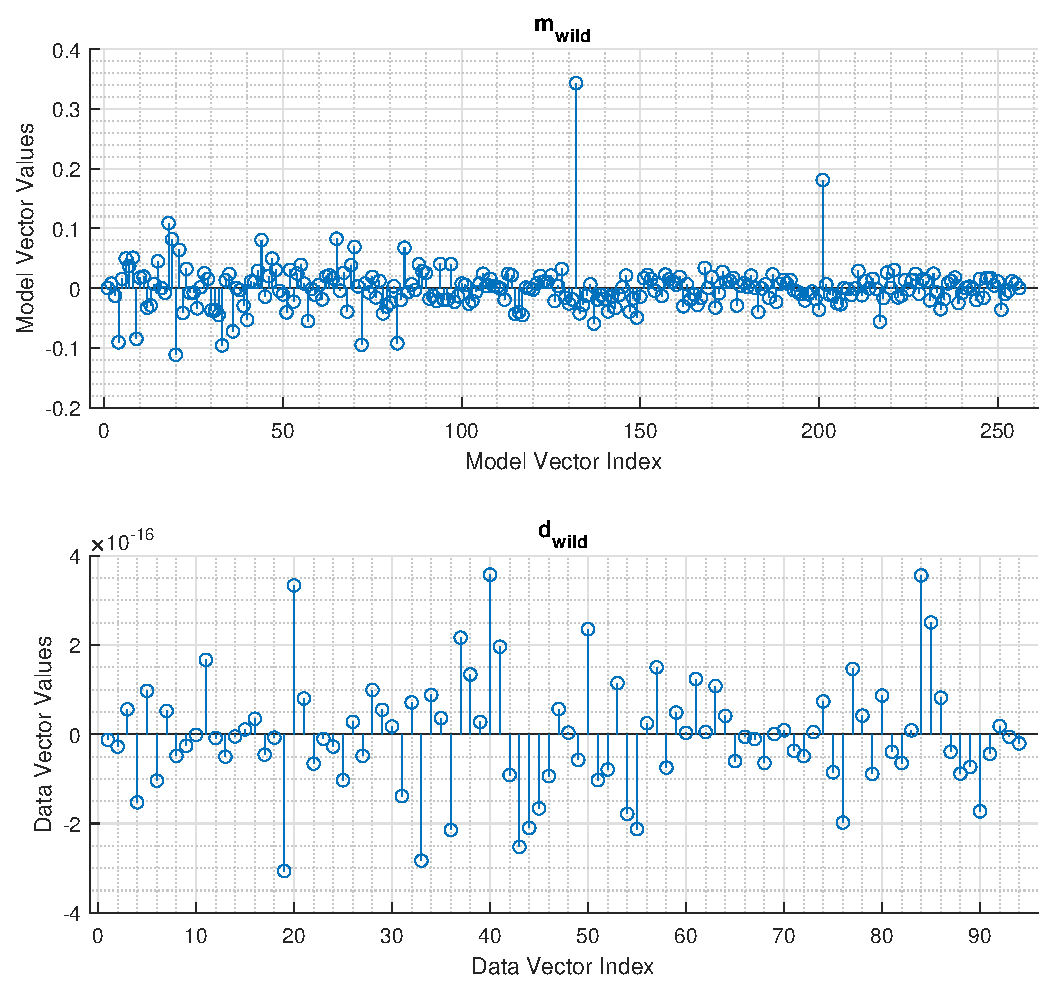
\includegraphics[width=0.85\textwidth]{./images/prob2_partB_wild_model_and_data.eps}
	\caption{Wild Model and Resulting Predicted Data}
	\label{fig: prob2 part B wild data and model}
\end{figure}
\FloatBarrier

Notice the scale of the values for the predicted data vector!

